% This version of CVPR template is provided by Ming-Ming Cheng.
% Please leave an issue if you found a bug:
% https://github.com/MCG-NKU/CVPR_Template.

\documentclass[final]{cvpr}
%\documentclass[reviewfinal]{cvpr}

\usepackage{times}
\usepackage{epsfig}
\usepackage{graphicx}
\usepackage{amsmath}
\usepackage{amssymb}
\usepackage{multirow} %表格多行
\usepackage{booktabs} %表格

% Include other packages here, before hyperref.

% If you comment hyperref and then uncomment it, you should delete
% egpaper.aux before re-running latex.  (Or just hit 'q' on the first latex
% run, let it finish, and you should be clear).
\usepackage[pagebackref,breaklinks,colorlinks]{hyperref}
\usepackage{fontspec}
\setmainfont{Times New Roman}

\def\cvprPaperID{123} % *** Enter the CVPR Paper ID here
\def\confName{ICCV}
\def\confYear{2021}
\graphicspath{{../assets/}}
%\setcounter{page}{4321} % For final version only


\begin{document}

%%%%%%%%% TITLE
\title{The Reading Report of Invertible Residual Networks}

\author{Yaqi Duan\\
South China University of Technology, Guangzhou, China\\
{\tt\small duanyaqiduanyaqi@gmail.com}
}

\maketitle


%%%%%%%%% ABSTRACT
\begin{abstract}
This article is a personal reading report\footnote {For more details about my own i-ResNet report. Please see: \url{https://github.com/DuanYaQi/iResNet}.}  of the Invertible Residual Networks. Different from the existing network architecture on the flow-based model, this paper propose a new invertible network based on the ResNet. This invertible network retains the easy-to-handle density estimation and non-volume preserving which is the flow-based model's advantages while eliminating the limits of the dimension division. Invertible ResNet uses a Lipschitz constraint to ingeniously solve the three problems of making the network invertible, calculating the network's inverse function, and log-determinant approximation. The invertible ResNet not only performs well in the generation task, but also shows the potential in the discrimination task.
\end{abstract}

%%%%%%%%% BODY TEXT
\section{Information}

This article is accepted by International Conference on Machine Learning, 2019. Invertible Residual Networks~\cite{behrmann2019invertible} is part of the innovation of Deep Learning Architectures system. The authors are Jens Behrmann, Will Grathwohl, Ricky T. Q. Chen, David Duvenaud, Jörn-Henrik Jacobsen from Universität Bremen, Germany, and Vector Institute, University of Toronto, Canada. By the way, Ricky T. Q. Chen, David Duvenaud are the authors of NeurIPS 2018 Best Paper-Neural Ordinary Differential Equations~\cite{chen2018neural}. And the Vector Institute is created by Geoffrey Hiton, received the 2018 Turing Award, together with Yoshua Bengio and Yann LeCun, for their work on deep learning.They are sometimes referred to as the "Godfathers of AI" and "Godfathers of Deep Learning".

%-------------------------------------------------------------------------
\section{Background}
First think about a question. Why do we need a invertible  model? The answer is a invertible model means information lossless, and the model can be used to make a better classification network, we can also use the maximum likelihood directly as a generative model. The work done in this article is based on the very powerful ResNet~\cite{he2016deep}, which means that it may have better performance than the previous flow-based model Glow~\cite{kingma2018glow} .

All in all, if a model is invertible , with low cost of reversibility and the strong ability of transform, then it can be used in discriminant tasks, density estimation, generation tasks and so on.

%------------------------------------------------------------------------
\subsection{Invertible Network Architecture}
Existing invertible network architectures, such as NICE~\cite{dinh2014nice}, RealNVP~\cite{dinh2016density}, and Glow~\cite{kingma2018glow}, achieve the reversibility of the model through clever dimensional decomposition of network architecture design. And by constraining the Jacobian matrix to be a triangular matrix to ensure the calculation cost of the determinant calculation, to further calculate the exactly log-likelihood. Though these model are elegant and beautiful in theory, there is a serious problem: because of the simple inverse transformation process, and the constraint of the Jacobian determinant, it will lead to weak nonlinear transformation capabilities in each layer.

The state-of-the-art flow-based model like Glow~\cite{kingma2018glow} , only transform a half of the variables in each layer. In order to ensure sufficient fitting capabilities, Glow~\cite{kingma2018glow} are higher requirements for the depth of the model (e.g. for 256-dimensional face generation tasks, the model uses about 600 convolutional layers, with a parameter amount of 200 M), and the calculation of this part is very large. However, invertible ResNet~\cite{behrmann2019invertible} doesn't require the deep number of network layers, it can still maintain sufficient transform capabilities with its architecture.

%------------------------------------------------------------------------
\subsection{Neural Ordinary Differential Equations}
The view of deep networks as dynamic over time provides two basic learning methods. One of them use discrete architecture to directly learn dynamics (Haber et al.~\cite{haber2017stable}; Ruthotto et al.~\cite{ruthotto2019deep}); the other (Chen et al.~\cite{chen2018neural}; Grathwohl et al.~\cite{grathwohl2019scalable}) use neural network parameterizes ordinary differential equations to indirectly learn dynamics. They usually regard the reversible transformation as a dynamic system that is approximated by an ordinary differential equation (ODE) solver.

The state-of-the-art NFs model Continuous  Normalizing Flows method (Chen et al.~\cite{chen2018neural})  use the Jacobian trace instead of the Jacobian determinant. The specific method is to parameterize the linear transformation process through an ordinary differential equation. But compared with invertible ResNet~\cite{behrmann2019invertible}, it does not have a fixed calculation budget. As shown in Figure \ref{fig:1}, the difference between the continuous dynamics of linearly invertible ResNet and the continuous dynamics of standard ResNet is explained. Invertible ResNets are bijective along continuous paths, while regular ResNets may result in crossing and collapsing paths.


%-------------------------------------------------------------------------3.
\section{Methodology}
The basic module of the ResNet model is

\begin{equation}
   y = x + g(x)\triangleq F(x)\label{eq1}
\end{equation}


where $x$ is the input feature, which is the identity mapping part, $g(x)$ is the feature transform, which is the residual part, and $y$ is the output feature. We call the Equation (\ref{eq1}) a ResNet Block. ResNet Block changes the original function $y$ into $y-x$, which the neural network needs to fit, and the $x,y$ are all vectors (tensors). 

This operation can ensure that the depth of the network is as large as possible, but there is no need to worry about the gradient dispersion. In a broad sense, ResNet allows the dimensionality to be changed by $1\times 1$ convolution, but here the ResNet does not change the dimensionality, means the input and output dimensions are the same, which is a necessary and sufficient condition for the bijective function.

For the classification problem, we only need to ensure that the network model is reversible, so as to achieve information lossless, see Section \ref{sec31}. For the reconstruction of the target, we need to calculate the inverse function of the network model for sampling and inference, see Section \ref{sec32}. For using maximum likelihood (the essence of the generation problem) models like flow-based model (e.g. NICE~\cite{dinh2014nice}, RealNVP~\cite{dinh2016density}, and Glow~\cite{kingma2018glow}) to train the generative model, then we need to solve the problem of the calculation loss of the Jacobian in the network, see Section \ref{sec33}.

\begin{figure}[t]
   \begin{center}
      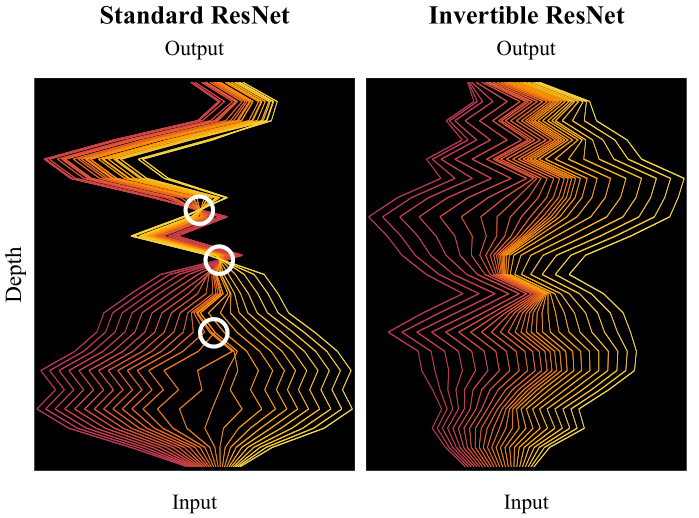
\includegraphics[width=1.0\linewidth]{1621241932669.png}
   \end{center}
      \caption{The dynamics of the standard ResNet network (left) and iResNet (right). Invertible ResNets describes a bijective continuous dynamics, while ResNets result in crossing and folding paths (circled in white) corresponding to non-bijective continuous dynamics. Due to the collapsing path, ResNets is not an effective density model.}
   \label{fig:1}
\end{figure}

\begin{figure*}[t]
   \begin{center}
      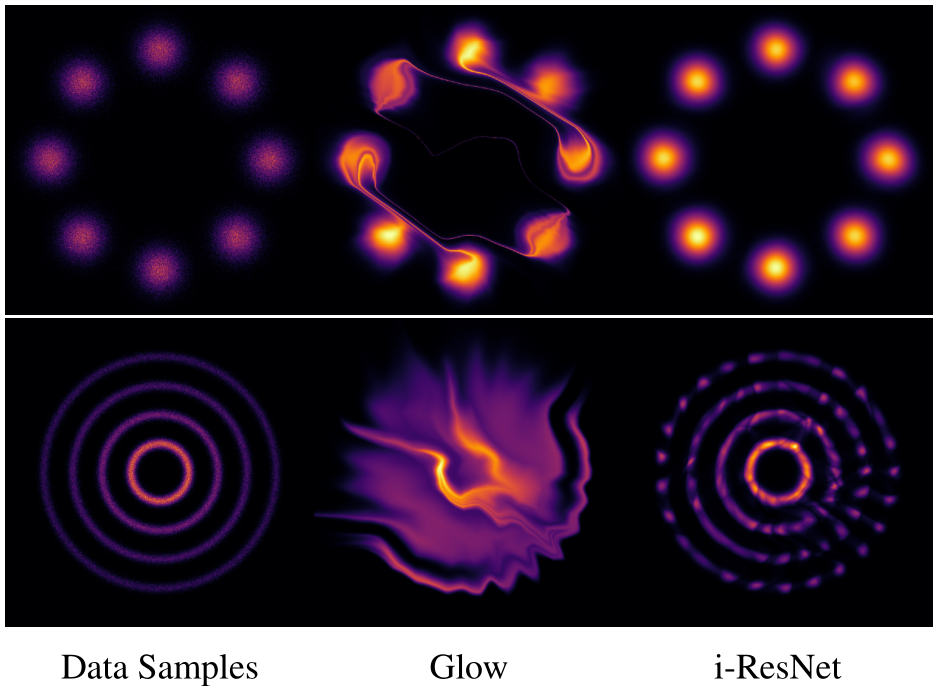
\includegraphics[width=0.7\linewidth]{1621944333639.png}
   \end{center}
      \caption{Visual comparison of i-ResNet flow and Glow.}
   \label{fig:2}
\end{figure*}

%------------------------------------------------------------------------3.1
\subsection{Invertible Condition}\label{sec31}
Equation \ref{eq1} is the basic module of ResNet, it is only necessary to ensure that each module is invertible . The sufficient condition for reversibility of Equation \ref{eq1} is

\begin{equation}
   \text{Lip}(g) <1
   \label{eq2}
\end{equation}

where $\text{Lip}(g) <1$ is the Lipschitz norm of the function $g$, and

\begin{equation}
   \text{Lip}(g) \triangleq \max_{x_1\neq x_2}\frac{\Vert g(x_1)-g(x_2)\Vert_2}{\Vert x_1-x_2\Vert_2}
   \label{eq3}
\end{equation}

The $g$ is a neural network, the neural network is a combination of matrix operations and activation functions,

\begin{equation}
   g(x)=\sigma(Wx+b)
\end{equation}

It is parameterized by the non-linear activation function $ \sigma$, and the affine transformation is represented by the weight $ W $ and the deviation $ b$. According to Equation \ref{eq3}, we have:


\begin{equation}
   \Vert \sigma(Wx_1+b)-\sigma(Wx_2+b)\Vert\leq C(W,b)\cdot \Vert x_1-x_2 \Vert
\end{equation}

where $C(W,b)$ is an expression about $W$ and $b$, and its value is Lipschitz constant. Let $\Delta x \to 0$ and use the first-order term approximation to get

\begin{equation}
   \left\Vert \frac{\partial \sigma}{\partial x}W(x_1-x_2)\right\Vert\leq C(W,b)\cdot \Vert x_1-x_2 \Vert
   \label{eq6}
\end{equation}

According to the chain rule, the sufficient condition for $\text{Lip}(g) <1$ is that the Lipschitz-Norm of $ \sigma$ is not more than 1 and the Lipschitz-Norm of $Wx+b$ is less than 1, so we have Condition \ref{eq7}

\begin{equation}
   \text{Lip}(\sigma)<1
   \quad \text{and} \quad
   \text{Lip}(Wx+b)<1
   \label{eq7}
\end{equation}

%------------------------------------------------------------------------3.1.1
\subsubsection{$\text{Lip}(\sigma)<1$}
To satisfies Condition \ref{eq7}. For the $\partial \sigma / \partial x$ term in Equation (\ref{eq6}), currently commonly used activation functions (such as sigmoid, tanh, relu, elu, etc.) all satisfy the constraint that the derivative has upper and lower bounds.

%------------------------------------------------------------------------3.1.2
\subsubsection{$\text{Lip}(Wx+b)<1$}
This term means that the Lipschitz-Norm of the matrix $W$ is required to be less than 1. Where the Lipschitz-Norm of the matrix $W$ is the Spectral-Norm, denoted as $\text{Lip}(W)$ or $\Vert W\Vert_2$.

To satisfies Condition \ref{eq7}. The Lipschitz-Norm of $Wx+b$ is less than 1, for the $W(x_1-x_2)$ term in Equation (\ref{eq6}), then we have

\begin{equation}
   \Vert W(x_1-x_2)\Vert\leq C\Vert x_1-x_2 \Vert
   \label{eq8}
\end{equation}

Now, the problem has been transformed into a matrix norm problem. The matrix norm is equivalent to the magnitude of the vector, which is defined as

\begin{equation}
   \Vert W\Vert_2 = \max_{x\neq 0}\frac{\Vert Wx\Vert}{\Vert x\Vert}
   \label{eq9}
\end{equation}

Equation (\ref{eq9}) also known as spectral norm, where $\Vert Wx\Vert$ and $\Vert x\Vert$ are the norms of vectors, the magnitude of the normal vector. According to Equation (\ref{eq9}), we convert Equation (\ref{eq8}) into

\begin{equation}
   \Vert W(x_1-x_2)\Vert\leq \Vert W\Vert_2\cdot\Vert x_1-x_2 \Vert
   \label{eq10}
\end{equation}

Note: I also find that Equation (\ref{eq10}) can also be proved by Cauchy's inequality transformation of Frobenius norm. And we can get that $\Vert W\Vert_F$ provides an upper bound of $\Vert W\Vert_2$. If accuracy is not required, you can also directly use $\Vert W\Vert_2 \to \Vert W\Vert_F$ to approximate and simplify calculation.\\

\noindent \textbf{Theorem 1}

The spectral norm $\Vert W\Vert_2$ is equal to the square root of the max eigenvalue (primary eigenvalue) of $W^{\top}W$. If $W$ is a square matrix, then $\Vert W\Vert_2$ is equal to The absolute value of the max eigenvalue of $W$. The proofs are given in Appendix [\ref{app1}].\\


According to Theorem 1, the problem is to find the max eigenvalue of $W^{\top}W$. invertible ResNet use the power iteration algorithm (see Appendix [\ref{app2}]) to calculate the max eigenvalue of $W^{\top}W$. It's also the spectral norm $\Vert W\Vert_2$, which takes the square of the spectral norm $\Vert W\Vert_2$ as an additional regular term

\begin{equation}
   loss = loss(y, g(x)) + \lambda \Vert W\Vert_2^2
   \label{eq11}
\end{equation}

The above Equation (\ref{eq11}) want to reduce to the smallest possible term $C=\Vert W\Vert_2$, so that the neural network satisfies the constraint of $\text{Lip}(Wx+b)<1$. Invertible Resnet adds this regular term to all the kernel weights $W$ in the model $g$ to make the entire network invertible.

%------------------------------------------------------------------------3.2.
\begin{table*}[]
   \caption{Comparison of i-ResNet to a ResNet-164 baseline architecture of similar depth and width with varying Lipschitz constraints via
   coefficients c. Vanilla shares the same architecture as i-ResNet, without the Lipschitz constraint.}
   \label{table1}   

   \begin{center}
   \begin{tabular}{@{}ccccccccc@{}}
   \toprule
                      &          & ResNet-164 & Vanila & c=0.9 & c=0.8 & c=0.7 & c=0.6 & c=0.8 \\ \midrule
   Classfication      & MNIST    & -          & 0.38   & 0.40  & 0.42  & 0.40  & 0.42  & 0.86  \\
   Error \%           & CIFAR10  & 5.50       & 6.69   & 6.78  & 6.86  & 6.93  & 7.72  & 8.71  \\
                      & CIFAR100 & 24.30      & 23.97  & 24.58 & 24.99 & 25.99 & 27.30 & 29.45 \\
                      \midrule
   Guaranteed Inverse &          & No         & No     & Yes   & Yes   & Yes   & Yes   & Yes   \\ \bottomrule
   \end{tabular}
   
\end{center}
\end{table*}




\subsection{Invertible Function Calculation}\label{sec32}
In order to further sample and inference for reconstructing the target. We also need to calculate the inverse function of the network.

Assume $y = x +g(x)$ is reversible, its implicit inverse function is $x = h(y)$, which is essentially to solve a system of nonlinear equations. The following iterative form is used in invertible Resnet

\begin{equation}
   x_{n+1}=y-g(x_n)
   \label{eq12}
\end{equation}

Obviously, the iterative sequence $\{x_n\}$ is related to $y$, and once $\{x_n\}$ converges to a fixed function

\begin{equation}
   \lim_{n\to\infty} x_n(y) = \hat{h}(y)
\end{equation}

we will have $\hat{h}(y)=yg\left(\hat{h}(y)\right)$, which means that $\hat{h}(y)$ is the requested $ x = h(y)$.

So if Equation (\ref{eq12}) converges, then the result of convergence is the inverse function of $x+g(x)$. We have

\begin{equation}
   \forall x_1,x_2,\quad\Vert g(x_1)-g(x_2)\Vert_2\leq \text{Lip}(g)\Vert x_1-x_2\Vert_2
\end{equation}

So according to Equation (\ref{eq2}), we have
\begin{equation}
   \begin{aligned}
      \Vert x_{n+1}-x_{n}\Vert_2&=\Vert g(x_{n})-g(x_{n-1})\Vert_2\\
&\leq \text{Lip}(g)\Vert x_{n}-x_{n-1}\Vert_2\\
& = \text{Lip}(g)\Vert g(x_{n-1})-g(x_{n-2})\Vert_2\\
&\leq \text{Lip}(g)^2\Vert x_{n-1}-x_{n-2}\Vert_2\\
&\dots\\
&\leq \text{Lip}(g)^n\Vert x_{1}-x_{0}\Vert_2\\
   \end{aligned}
\end{equation}

According to Banach's fixed point theorem, we have a sufficient condition of $\Vert x_{n+1}-x_{n}\Vert_2\to 0$ is $\text{Lip}(g) <1$. The content of Cauchylie is involved, and the proofs are given in Appendix [\ref{app3}].

When the normalization operation is done to make $x+g(x)$ reversible, its inverse function is the fixed point of $x_{n+1}=y-g(x_n)$. In the numerical calculation, only need to use the Equation (\ref{eq12}) iterative format to iterate a certain number of steps, so that the accuracy satisfy the requirements, and the convergence result can be obtained, which is the inverse function of $x+g(x)$.

%------------------------------------------------------------------------3.3.


\subsection{Jacobian Determinant Calculation}\label{sec33}
In order to use the maximum likelihood (the essence of the generation problem) as the loss function to train the generative model, for learning the powerful generative ability. It is necessary to calculate the Jacobian determinant. First, calculate the Jacobian matrix:

\begin{equation}
   J_F\triangleq \frac{\partial}{\partial x}(x+g(x)) = I + \frac{\partial g}{\partial x}\triangleq I + J_g
\end{equation}

The Jacobian determinant is $\det(J_F)=\det (I+J_g)$, but in fact, when training generative models, we alway calculate the logarithm of the absolute value of the Jacobian determinant,which is

\begin{equation}
   \ln |\det(J_F)| = \ln |\det(I + J_g)|\equiv \ln \det(I + J_g)
   \label{eq17}
\end{equation}

The reason for eliminating the absolute value here is that the disturbance of the Lipschitz constraint identity makes $x + g(x)$ produce a constant positive determinant.\\


\noindent \textbf{Theorem 2}

\begin{equation}
   \ln\det(\boldsymbol{A}) = \text{Tr}(\ln (\boldsymbol{A}))
\end{equation}

\noindent The proofs are given in Appendix [\ref{app1}].\\


We can't calculate the Jacobian by Equation (\ref{eq17}), because the amount of calculation is too large, and when backpropagating, the derivative of the determinant must be calculated, which is more complicated. Invertible Resnet came up with a cumbersome but effective solution, and uses Theorem 2 to get the following formula


\begin{equation}
   \ln\det(I + J_g) = \text{Tr}(\ln (I+J_g))
\end{equation}
   

\noindent Expand $\ln (I+J_g)$ by the logarithmic expansion of the real series as:

\begin{equation}
   \ln (I + J_g) = \sum_{n=1}^{\infty}(-1)^{n-1}\frac{J_g^n}{n}
   \label{eq20}
\end{equation}

The condition for the convergence of the series is $\Vert J_g\Vert_2 <1$, $\text{Lip}(g) <1$, which is exactly the constraint of invertible Resnet.

Now $\ln (I + J_g)$ is an infinite series. If the $n$ term is truncated, then the error is proportional to $\text{Lip}(g)^n$, so invertible Resnet is based on $\text{Lip} (g)$ to determine the number of truncation. we can further write:

\begin{equation}
   \text{Tr}(\ln (I + J_g)) = \sum_{n=1}^{N}(-1)^{n-1}\frac{\text{Tr}(J_g^n)}{n}+O\left(\text{Lip}(g)^N\right)
   \label{eq21}
\end{equation}

The Equation (\ref{eq21}) needs to calculate $J_g^n$. But the $J_g$ is a matrix, and the cost of calculating the matrix to the power of $n$ is too huge. Therefore, invertible Resnet assumes that for any matrix $A$, there is

\begin{equation}
   \text{Tr}(A)=\mathbb{E}_{u\sim p(u)}\big[u^{\top}Au\big]
   \label{eq22}
\end{equation}

where $p(u)$ is a multivariate probability distribution, its mean is 0, and the covariance is the identity matrix. Invertible Resnet randomly selects a vector $u$ from $p(u)$ for each iteration, and then make that $u^{\top}Au$ is $\text{Tr}(A)$, i.e. transforms Equation (\ref{eq21}) to Equation (\ref{eq23})

\begin{equation}
   \text{Tr}(\ln (I + J_g)) \approx \sum_{n=1}^{N}(-1)^{n-1}\frac{u^{\top } J_g^nu}{n},\quad u\sim p(u)
   \label{eq23}
\end{equation}

where

\begin{equation}
   u^{\top} J_g^n u=u^{\top} J_g(\dots(J_g(J_g u)))
\end{equation}

Therefore, we don't need to calculate $J_g^n$, and each step we only need to calculate the multiplication of a matrix and a vector, and each step of the calculation can be reused, so the cost of calculation is greatly reduced.
\begin{figure}
   \begin{center}
   
      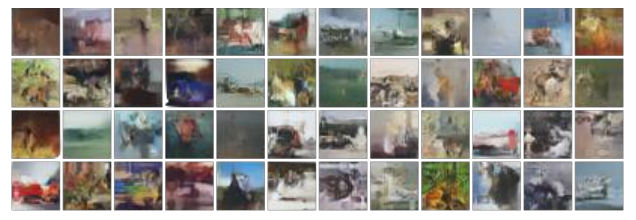
\includegraphics[width=1.0\linewidth]{image-20210526232348670.png}
   \end{center}
      \caption{CIFAR10 samples from our i-ResNet flow.}
   \label{fig:4}
\end{figure}
Invertible Resnet first perform logarithmic expansion of the Jacobian matrix with Equation (\ref{eq20}), and then convert the determinant calculation into the trace calculation with Equation (\ref{eq21}), and use the probability sampling method with Equation (\ref{eq22}), the Jacobian can be calculated most efficiently.


%------------------------------------------------------------------------4.
\begin{table}[]
   \caption{MNIST and CIFAR10 bits/dim results. $†$ Uses ZCA pre-processing making results not directly comparable.}
   \label{table2}
   \begin{center}
      \begin{tabular}{@{}lcc@{}}
         \toprule
         Method                          & MNIST & CIFAR10 \\ \midrule
         NICE (Dinh et al.~\cite{dinh2014nice})        & 4.36  & 4.48$†$ \\
         MADE (Germain et al.~\cite{germain2015made})     & 2.04  & 5.67    \\
         MAF (Papamakarios et al.~\cite{papamakarios2017masked}) & 1.89  & 4.31    \\
         Real NVP (Dinh et al.~\cite{dinh2016density})    & 1.06  & 3.49    \\
         Glow (Kingma \& Dhariwal~\cite{kingma2018glow}) & 1.05  & 3.35    \\
         FFJORD (Grathwohl et al.~\cite{grathwohl2019scalable}) & 0.99  & 3.40    \\ \midrule
         i-ResNet~\cite{behrmann2019invertible} & 1.06  & 3.45    \\ \bottomrule
         \end{tabular}
   \end{center}
\end{table}


\section{Results}

%------------------------------------------------------------------------4.1
\subsection{Toy Dataset Experiment}
The Toy data set constructs some regular random points. The purpose is to use a generative model to fit its distribution. Such experiments are often done in GAN. From the Figure \ref{fig:2}, you can see that the effect of invertible Resnet~\cite{behrmann2019invertible} is much better than Glow~\cite{kingma2018glow}. I think it’s because invertible Resnet is a very symmetrical model with no bias in dimension, while Glow is biased in dimension. It requires us to shuffle the input in some way, and then split it in half. Different, which brings about the problem of asymmetry.

%------------------------------------------------------------------------4.2



\subsection{Discrimination Task Experiment}
Since invertible Resnet is a network based on ResNet, its most basic use is for classification task. Table \ref{table1} shows that using invertible Resnet~\cite{behrmann2019invertible} for classification tasks, the effect is also very good, the existence of Lipschitz constraints will not significantly affect the classification results ($c$ equals $\text{Lip}(g)$).


Where ResNet-164 is a network with an architecture similar to invertible Resnet, and vanilla represents ResNet without Lipschitz constraints. It is observed that when a very conservative normalization is applied (when $c$ is very small), the classification error of all tested data sets will be higher, but when $c$ is large, espically it approaches 1, which is compared with ordinary ResNet-64 is extremely competitive.

%------------------------------------------------------------------------4.3
\subsection{Generative model experiment}
The state-of-the-art flow-based model series is poorer than GAN in terms of generating complex pictures, but the quantitative comparison between them has no obvious advantages and disadvantages. We compare invertible Resnet with it, replace the coupling layer in the flow-based model with reversible residual blocks that have the same number of parameters, and replace the reversible linear transformation with Actnorm (Kingma et al.~\cite{kingma2018glow}). Figure \ref{fig:4} shows that the invertible Resnet is also excellent as a flow-based generative model.

The comparison with the results of other generative models can be found in Table \ref{table2}. Although the invertible Resnet is not as good as Glow~\cite{kingma2018glow} and FFJORD~\cite{grathwohl2019scalable}, it is surprising that ResNets can be created to compete with these highly engineered generative models with very few modifications.


%------------------------------------------------------------------------


\section{Conclusion}
Before invertible Resnet, one of the most successful feed-forward architectures for discriminative learning was the deep residual network~\cite{he2016deep}, but this architecture is very different from the corresponding generative model. This division complicates the selection or design of the appropriate architecture for a given task. And invertible Resnet proposes a new architecture with good performance that can solve this problem and bridges this gap. And it is not limited to specific network structure design. The whole work is very violent. Through a Lipschitz constant, the three problems of the reversible maximum likelihood generation model are solved. There is a whole sense of beauty in it.

However, there is still a gap between the results of individual networks in the discrimination task and the generation task. I think this is because the author is calculating the matrix trace Equation (\ref{eq21}) using the method of probability sampling Equation (\ref{eq22}), only taking a vector $u$ randomly from the multivariate probability distribution $p( u)$, which leads to a biased estimate of the logarithmic determinant~\cite{han2018stochastic}. I personally think that if this part of the estimate can be processed by an unbiased method~\cite{anil2019sorting}, it may improve certain performance.


%-------------------------------------------------------------------------


% Update the cvpr.cls to do the following automatically.
% For this citation style, keep multiple citations in numerical (not
% chronological) order, so prefer \cite{Alpher03,Alpher02,Authors14} to
% \cite{Alpher02,Alpher03,Authors14}.



{\small
\bibliographystyle{ieee_fullname}

\bibliography{egbib}
}


%------------------------------------------------------------------------ appendix
\clearpage
\begin {appendix}
\section{Additional Lemmas and Proofs}
\label{app1}
\noindent\emph{Proof}. (\textbf{Theorem 1})

According to Equation (\ref{eq9}), we have

\begin{equation}
\Vert W\Vert_2^2 = \max_{x\neq 0}\frac{x^{\top}W^{\top} Wx}{x^{\top} x} = \max_{\Vert x\ Vert=1}x^{\top}W^{\top} Wx
\end{equation}

Suppose $W^{\top} W$ is diagonalized to $\text{diag}(\lambda_1,\dots,\lambda_n)$, that is, $W^{\top} W=U^{\top}\text {diag}(\lambda_1,\dots,\lambda_n)U$, where $\lambda_i$ are all its characteristic roots and non-negative, where $U$ is an orthogonal matrix, due to the product of orthogonal matrix and unit vector Or unit vector, then

\begin{equation}
\begin{aligned}\Vert W\Vert_2^2 =& \max_{\Vert x\Vert=1}x^{\top}\text{diag}(\lambda_1,\dots,\lambda_n) x \\
=& \max_{\Vert x\Vert=1} \lambda_1 x_1^2 + \dots + \lambda_n x_n^2\\
\leq & \max\{\lambda_1,\dots,\lambda_n\} (x_1^2 + \dots + x_n^2)\quad(\text{Note:}\Vert x\Vert=1)\\
=&\max\{\lambda_1,\dots,\lambda_n\}\end{aligned}
\end{equation}

Thus $\Vert W\Vert_2^2$ is equal to the largest characteristic root of $W^{\top} W$.
\\
\\
\\
\noindent\emph{Proof}. (\textbf{Theorem 2})

We consider the scalar parameter $t$

\begin{equation}f(t)=\det(\exp(t\boldsymbol{A}))\end{equation}

Then find its derivative to get

\begin{equation}\begin{aligned}\frac{d}{dt}f(t)=&f(t)\text{Tr}\left(\exp(-t\boldsymbol{A})\underbrace{\ frac{d}{dt}\exp(t\boldsymbol{A})}_{=\exp(t\boldsymbol{A})\boldsymbol{A}}\right)\\
=&f(t)\text{Tr}(\boldsymbol{A})\end{aligned}\end{equation}

Where $\text{Tr}(\boldsymbol{A})$ is a constant, we get a first-order homogeneous differential equation. Its analytical solution is

\begin{equation}f(t)=C\exp(t\,\text{Tr}(\boldsymbol{A}))\end{equation}

When $t=0$, we have $f(0)=1$, and further calculations get $C=1$, that is, $f(t)=\exp(t\,\text{Tr}(\boldsymbol{ A}))$, which proves

\begin{equation}\det(\exp(t\boldsymbol{A}))=\exp(t\,\text{Tr}(\boldsymbol{A}))\end{equation}

When $t=1$, the identity $\det(\exp(\boldsymbol{A})) = \exp(\text{Tr}(\boldsymbol{A}))$ is obtained. Take the logarithm on both sides, you can get another common form of it

\begin{equation}\ln\det(\boldsymbol{B}) = \text{Tr}(\ln (\boldsymbol{B}))\end{equation}


%------------------------------------------------------------------------
\section{Power iterations Algorithm}
\label{app2}
Power iteration through the above iteration format

\begin{equation}u \leftarrow \frac{(W^{\top}W)u}{\Vert (W^{\top}W)u\Vert}\end{equation}

After several iterations, the following formula is finally passed

\begin{equation}\Vert W\Vert_2^2\approx u^{\top}W^{\top}Wu\end{equation}

Get the norm, which is the approximate value of the largest characteristic root. It can also be equivalently rewritten as

\begin{equation}v\leftarrow \frac{W^{\top}u}{\Vert W^{\top}u\Vert},\,u\leftarrow \frac{Wv}{\Vert Wv\Vert} ,\quad \Vert W\Vert_2 \approx u^{\top}Wv\end{equation}

In this way, after initializing $u,v$ (it can be initialized with a vector of all 1s), you can iterate several times to get $u,v$, and then substituting $u^{\top}Wv$ into $\Vert W\Vert_2$ approximation.

%------------------------------------------------------------------------
\section{Banach's Fixed Point Theorem}
\label{app3}
For any positive integer $k$, we continue to consider $\Vert x_{n+k}-x_{n}\Vert_2$:

\begin{equation}\begin{aligned}\Vert x_{n+k}-x_{n}\Vert_2&\leq\Vert x_{n+k}-x_{n+k-1}\Vert_2+\dots\\&+\Vert x_{n+2}-x_{n+1}\Vert_2+\Vert x_{n+1}-x_{n}\Vert_2\\
&\leq \left(\text{Lip}(g)^{n+k-1}+\dots +\text{Lip}(g)^{ n}\right)\Vert x_{1}-x_{0}\Vert_2\\
& = \frac{1-\text{Lip}(g)^k}{1-\text{Lip}(g)}\cdot\text{Lip}(g)^{n}\Vert x_{1} -x_{0}\Vert_2\\
& \leq \frac{\text{Lip}(g)^n}{1-\text{Lip}(g)}\Vert x_{1}-x_{0}\Vert_2
\end{aligned}\end{equation}

It can be seen that we have got an upper bound of $\Vert x_{n+k}-x_{n}\Vert_2$, which is only related to $n$ and can be arbitrarily small. In other words, for any $\varepsilon> 0$, we can find a $n$ such that for any positive integer $k$ there is $\Vert x_{n+k}-x_{n}\Vert_2 <\ varepsilon$. We call this sequence of numbers the Cauchy sequence, and it is bound to converge. At this point, we finally proved the convergence.

By the way, in the above formula, taking $k\to\infty$, we get:

\begin{equation}\left\Vert x^*-x_{n}\right\Vert_2 \leq \frac{\text{Lip}(g)^n}{1-\text{Lip}(g)}\ Vert x_{1}-x_{0}\Vert_2\end{equation}

In other words, the convergence speed of this iterative algorithm is proportional to $\text{Lip}(g)^n$, so naturally, the smaller the $\text{Lip}(g)$, the faster the convergence, but $\text{ The smaller Lip}(g)$, the weaker the fitting ability of the model. In the original paper, its range is $0.5-0.9$.

To be more ambitious, this is actually the Banach fixed point theorem in functional analysis, also known as the compression mapping theorem (because $\text{Lip}(g)$ is less than 1, so $g$ is called Is a compression map.).

\end {appendix}


\end{document}
